\paragraph{}
Rappelons d'abord brievement ce qu'est une chaîne de Markov. Une chaîne de Markov est un outil mathématique stochastique, qui utilise un principe de "non-mémoire". Tout état d'un système est simplement calculé à partir du précédent, ce qui en facilite l'analyse.
\\\\
Ces chaînes sont simplement décrites mathématiquement comme suit avec $X_1, X_2,..., X_t$ une suite de variables aléatoires qui définit une chaîne de Markov
si (pour t > 1) elle suit cette relation :
\begin{equation*}
  \mathbb{P}(X_1, X_2, ..., X_t) = \mathbb{P}(X_1)\prod_{l = 2}^{t}\mathbb{P}(X_l | X_{l-1}) 
\end{equation*}

\subsubsection{}

Nous calculons donc pour des valeurs de $t$ croissantes les différentes valeurs demandées, ici avec $t = 20$ (suffit pour avoir convergé) :
\begin{itemize}
  \item Cas de base distribué uniformément : $\mathbb{P}(X_t = x) = 
  \begin{pmatrix}
    0.3488 & 0.0698 & 0.2326 & 0.3488\\
  \end{pmatrix}$ avec $x = 1, 2, 3, 4$
  \item Cas de base fixé : $\mathbb{P}(X_t = x) = 
  \begin{pmatrix}
    0.3488 & 0.0698 & 0.2326 & 0.3488\\
  \end{pmatrix}$ avec $x = 1, 2, 3, 4$
  \item $Q^t = 
  \begin{pmatrix}
  0.3488 & 0.0698 & 0.2325 & 0.3488\\
  0.3488 & 0.0698 & 0.2326 & 0.3488\\
  0.3488 & 0.0698 & 0.2326 & 0.3488\\
  0.3488 & 0.0698 & 0.2326 & 0.3488\\
  \end{pmatrix}$ 
\end{itemize}

On remarque donc bien une convergence vers des probabilités et ceci peut importe le cas de départ, on peut montrer cette convergence sur les figures ci-dessous :
\begin{figure}[h!]
  \centering
  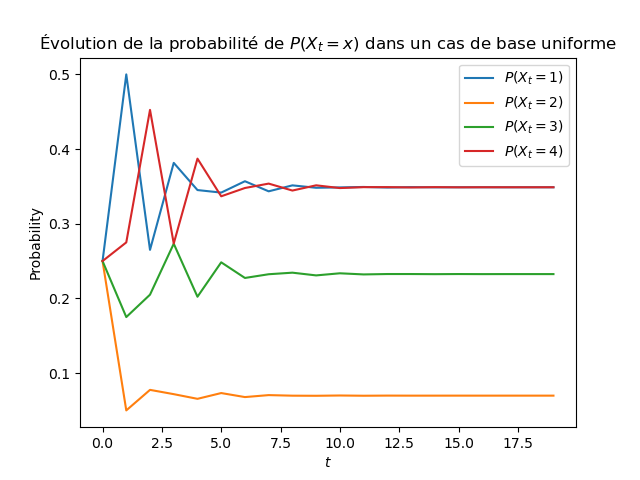
\includegraphics[width=0.5\textwidth]{figs/evo_unif.png}
  \caption{Évolution des probabilités dans une distribution de départ uniforme}
\end{figure}
\\
\begin{figure}[h!]
  \centering
  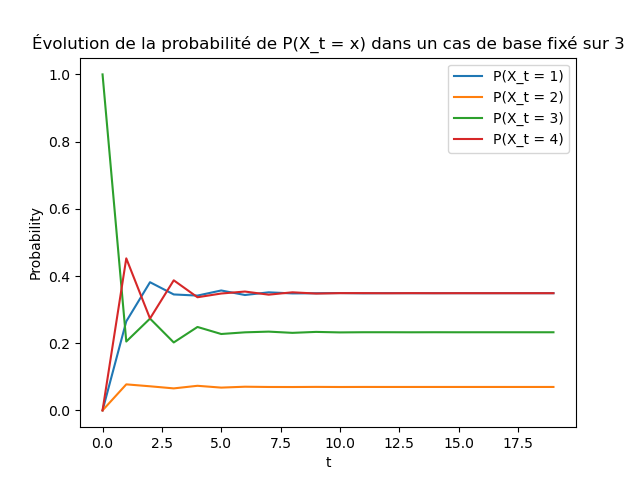
\includegraphics[width=0.5\textwidth]{figs/evo_fixed.png}
  \caption{Évolution des probabilités dans une distribution de départ fixée sur 3}
\end{figure}

\subsubsection{}

Afin de déduire la distribution stationnaire $\pi_{\infty}$ de notre chaîne qui est décrite comme suit :
\begin{equation*}
  [\pi_\infty]_j = \lim_{t \rightarrow \infty} \mathbb{P}(X_t = j)
\end{equation*}

Nous allons simplement calculer $\mathbb{P}(X_t)$ avec un grand $t$ ce qui nous donne :
\begin{equation*}
  \pi_{\infty} = 
  \begin{pmatrix}
    0.3488 & 0.0698 & 0.2326 & 0.3488
  \end{pmatrix}
\end{equation*}

\subsubsection{}
Afin de vérifier les résultats obtenus, nous effectuons des réalisations de notre chaîne de Markov. Nous pouvons mettre en tableau la proportion de réalisation 
de chaque état lors de tests avec un nombre de pas croissant. Nous utilisons un point de départ distribué uniformément entre les 4 états car il a été prouvé
plus haut que ça n'avait pas d'influence.

\begin{table}[h!]
  \begin{tabular}{|c|c|c|c|c|}
  \hline
  \# Pas / État & \multicolumn{1}{c|}{1} & \multicolumn{1}{c|}{2} & \multicolumn{1}{c|}{3} & 4 \\ \hline
  100     & 0.35    & 0.05   & 0.21    & 0.39    \\ \hline
  1000    & 0.351   & 0.075  & 0.23    & 0.344   \\ \hline
  10000   & 0.346   & 0.064  & 0.236   & 0.354   \\ \hline
  100000  & 0.3501  & 0.0722 & 0.228   & 0.3497  \\ \hline
  1000000 & 0.34902 & 0.6757 & 0.23422 & 0.34919 \\ \hline
  \end{tabular}
  \centering
  \caption{Proportion des états obtenus en fonction de nombre de pas}
  \label{tab:table-prop}
\end{table}

En comparant ce tableau avec les résultats obtenus avec les valeurs précédement obtenus, on remarque bien que les proportions sont respectées et font sens, on converge bien 
vers les mêmes valeurs.

\subsubsection{}
/!$\backslash$ TODO /!$\backslash$